\documentclass[12pt,compress,aspectratio=169]{beamer}
\usetheme{metropolis}
\setbeamersize{text margin left=.5cm,text margin right=.5cm}
\usepackage[lf]{carlito}
\usepackage{siunitx}
\usepackage{tikz}
\usepackage{mathpazo}
\usepackage{bm}
\usepackage{mathtools}
\usepackage[ISO]{diffcoeff}
\diffdef{}{ op-symbol=\mathsf{d} }
\usepackage{xcolor,colortbl}

\setmonofont{Ubuntu Mono}
\setlength{\parskip}{0pt}
\renewcommand{\baselinestretch}{1}

\sisetup{
  inter-unit-product=\cdot,
  per-mode=symbol
}

\tikzset{
  >=latex
}

%\newcommand{\iii}{\hat{\bm\imath}}
%\newcommand{\jjj}{\hat{\bm\jmath}}
%\newcommand{\kkk}{\hat{\bm k}}


\usetikzlibrary{decorations.pathmorphing,patterns}

\setmonofont{Ubuntu Mono}
\setlength{\parskip}{0pt}
\setlength{\itemsep}{0pt}
\renewcommand{\baselinestretch}{1}

\sisetup{
  per-mode=symbol
}
\tikzset{>=latex}

\title{Topic 5a: Gravity}
\subtitle{AP and IBHL Physics}
\author[TML]{Dr.\ Timothy Leung}
\institute{Olympiads School}
\date{Updated: Summer 2022}

\newcommand{\pic}[2]{
  \includegraphics[width=#1\textwidth]{#2}
}
\newcommand{\eq}[2]{
  \vspace{#1}{\Large
    \begin{displaymath}
      #2
    \end{displaymath}
  }
}
%\newcommand{\iii}{\ensuremath\hat{\bm{\imath}}}
%\newcommand{\jjj}{\ensuremath\hat{\bm{\jmath}}}
%\newcommand{\kkk}{\ensuremath\hat{\bm{k}}}
\newcommand{\iii}{\ensuremath\hat\imath}
\newcommand{\jjj}{\ensuremath\hat\jmath}
\newcommand{\kkk}{\ensuremath\hat k}



\begin{document}

\begin{frame}
  \maketitle
\end{frame}



\section{Gravitational Force}

\begin{frame}{Law of Universal Gravitation}
  \begin{center}
    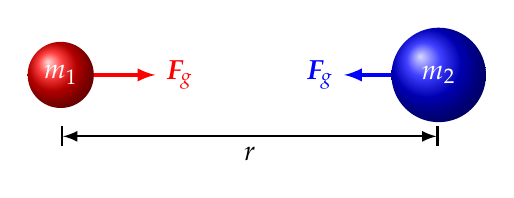
\begin{tikzpicture}[scale=.6]
      \draw[->,very thick,red] (0,0)--(2,0) node[right]{$\bm{F}_g$};
      \draw[->,very thick,blue](8,0)--(6,0) node[left] {$\bm{F}_g$};
      \tikzstyle{balloon1}=[ball color=red];
      \tikzstyle{balloon2}=[ball color=blue];
      \shade[balloon1] (0,0) circle(.7) node[white]{$m_1$};
      \shade[balloon2] (8,0) circle(1) node[white]{$m_2$};
      \draw[|<->|,thick](0,-1.3)--(8,-1.3)node[midway,below]{$r$};
    \end{tikzpicture}
  \end{center}
  In classical mechanics, \textbf{gravity} is a mutually attractive force
  between all massive objects; the magnitude $F_g$ is determined by the law of
  universal gravitation:

  \eq{-.2in}{
    \boxed{
      F_g=G\frac{m_1m_2}{r^2}
    }
  }

  where $G=\SI{6.674e-11}{\newton\metre\squared\per\kilo\gram\squared}$ is the
  \textbf{universal gravitation constant}, and $r$ is the distance between the
  centers of the masses. $m_1$ and $m_2$ are assumed to be \emph{point masses}
  that do not occupy any space.
\end{frame}



\begin{frame}{More Than One Mass}
  \begin{columns}
    \column{.4\textwidth}
    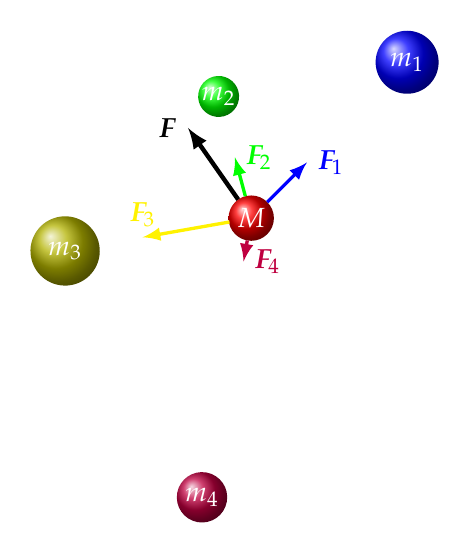
\begin{tikzpicture}[scale=.4]
      \tikzstyle{balloon1}=[ball color=red];
      \tikzstyle{balloon2}=[ball color=blue];
      \tikzstyle{balloon3}=[ball color=green];
      \tikzstyle{balloon4}=[ball color=yellow!70!black];
      \tikzstyle{balloon5}=[ball color=purple];
      \shade[balloon1] (0,0) circle(.72) node[white]{$M$};
      \begin{scope}[rotate=45]
        \draw[->,very thick,blue](.72,0)--(2.5,0) node[right]{$\bm{F}_1$};
        \shade[balloon2] (7,0) circle(1) node[white]{$m_1$};
      \end{scope}
      \uncover<2->{
        \begin{scope}[rotate=105]
          \draw[->,very thick,green](.72,0)--(2,0)
          node[right]{$\bm{F}_2$};
          \shade[balloon3] (4,0) circle(.65) node[white]{$m_2$};
        \end{scope}
      }
      \uncover<3->{
        \begin{scope}[rotate=190]
          \draw[->,very thick,yellow](.7,0)--(3.5,0)
          node[above]{$\bm{F}_3$};
          \shade[balloon4] (6,0) circle(1.1) node[white]{$m_3$};
        \end{scope}
      }
      \uncover<4->{
        \begin{scope}[rotate=260]
          \draw[->,very thick,purple](.72,0)--(1.4,0)
          node[right]{$\bm{F}_4$};
          \shade[balloon5] (9,0) circle(.8) node[white]{$m_4$};
        \end{scope}
      }
      \uncover<5>{
        \begin{scope}[rotate=125]
          \draw[->,ultra thick](.72,0)--(3.5,0) node[left]{$\bm{F}$};
        \end{scope}
      }
    \end{tikzpicture}

    \column{.6\textwidth}
    For a mass $M$ that is subjected to the influence of multiple discrete point
    masses $m_i$, the total gravitational force that $M$ experiences
    is the vector sum of all the forces $\bm{F}_i$:
    
    \eq{-.25in}{
      \boxed{\bm{F}
        =\sum_i\bm{F}_i
        =GM\left(\sum_{i=1}^N\frac{m_i}{r_i^2}\hat{\bm{r}_i}\right)
      }
    }
  \end{columns}
\end{frame}



\section{Gravitational Field}

\begin{frame}{Gravitational Field}
  We generally describe the gravitational force $\bm{F}_g$ (or weight $\bm{w}$)
  as:
  
  \eq{-.2in}{
    \boxed{\bm{w}=\bm{F}_g=m\bm{g}}
  }

  To find $\bm{g}$, we group the variables in the law of universal gravitation:
    
  \eq{-.2in}{
    \bm{F}_g
    =\underbrace{\left[-\frac{Gm_1}{|\bm{r}|^2}\hat{\bm{r}}\right]}_{=\bm{g}}m
    =m\bm{g}
  }

  The vector field function $\bm{g}$ is known as the
  \textbf{acceleration due to gravity} in kinematics, and
  \textbf{gravitational field} in field theory.
\end{frame}



\begin{frame}{Gravitational Field}
  On/near the surface of Earth, we can use Earth's mass and radius

  \vspace{-.4in}{\Large
    \begin{align*}
      m_1&=\SI{5.972e24}{\kilo\gram}\\
      r&=\SI{6.371e6}{\metre}
    \end{align*}
  }
  
  \vspace{-.2in}to compute the commonly known value of

  \vspace{-.4in}{\Large
    \begin{align*}
      g &\approx\SI{9.81}{\metre\per\second^2}\\
      g &\approx\SI{9.81}{\newton\per\kilo\gram}
    \end{align*}
  }
\end{frame}



\begin{frame}{Gravitational Field}
  The \textbf{gravitational field} $\bm{g}$ generated by point mass $m$
  shows how it influences the gravitational forces on other masses:

  \eq{-.2in}{
    \boxed{g(m,\bm{r})=-\frac{Gm}{|\bm{r}|^2}\hat{\bm{r}}}
  }
  \begin{center}
    \begin{tabular}{l|c|c}
      \rowcolor{pink}
      \textbf{Quantity} & \textbf{Symbol} & \textbf{SI Unit} \\ \hline
      Gravitational field       & $\bm{g}$ & \si{\newton\per\kilo\gram}\\
      Universal gravitational constant
      & $G$ & \si{\newton\metre^2/\kilo\gram^2} \\
      Source mass               & $m$ & \si{\kilo\gram} \\
      Distance from source mass & $|\bm{r}|$ & \si{\metre}\\
      Outward radial unit vector from source & $\hat{\bm{r}}$ & N/A
    \end{tabular}
  \end{center}
  The \emph{direction} of the gravitational field is toward $m$ (that's why the
  negative sign)
\end{frame}



\begin{frame}{More Than One Mass}
  When there are multiple point masses present, the total gravitational field
  at any position $\bm{r}$ is the vector sum of all the fields $\bm{g}_i$:
    
  \eq{-.2in}{
    \boxed{\bm{g}
      =\sum_i\bm{g}_i
      =G\left(\sum_i\frac{m_i}{r_i^2}\hat{\bm{r}_i}\right)
    }
  }
\end{frame}




\begin{frame}{Relating Gravitational Field \& Gravitational Force}
  $\bm{g}$ acts on any mass $m$ that enters the field. Then, $m$ experiences a
  gravitational force $\bm{F}_g$, regardless of how $\bm{g}$ is created:

  \eq{-.2in}{
    \boxed{\bm{F}_g=m\bm{g}}
  }
  \begin{center}
    \begin{tabular}{l|c|c}
      \rowcolor{pink}
      \textbf{Quantity} & \textbf{Symbol} & \textbf{SI Unit} \\ \hline
      Gravitational force on a mass & $\bm{F}_g$ & \si{\newton} \\
      Mass inside the gravitational field & $m$ & \si{\kilo\gram}\\
      Gravitational field & $\bm{g}$   & \si{\newton\per\kilogram}
    \end{tabular}
  \end{center}
  Note: A point mass is not affected by the gravitational field that itself
  generates.
\end{frame}



\begin{frame}{Gravitational Field Lines}
  \begin{center}
    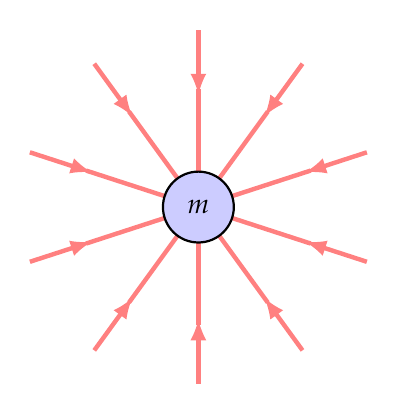
\begin{tikzpicture}[scale=1.5]
      \foreach \x in {0,...,9}{
        \draw[red!50,ultra thick,rotate=36*\x](0,0)--(0,1);
      }
      \foreach \x in {0,...,9}{
        \draw[red!50,<-,ultra thick,rotate around={36*\x:(0,0)}](0,.95)--(0,1.5);
      }
      \draw[fill=blue!20,thick](0,0) circle(.3) node{$m$};
    \end{tikzpicture}
  \end{center}
  \begin{itemize}
  \item The direction of $\bm{g}$ is toward the center of the object that
    created it
  \item Field lines do not tell the intensity (i.e.\ magnitude) of $\bm{g}$,
    only the direction
  \end{itemize}
\end{frame}



\begin{frame}{Gravitational Field Lines}
  When there are multiple masses, the total gravitational field (dotted line)
  is the vector sum of all the individual fields.
  \begin{center}
    \pic{.4}{grav-fields}
  \end{center}
  The solid lines are called \textbf{equipotential lines}, where the potential
  energy is constant. Equipotential lines are perpendicular to
  gravitational field lines.
\end{frame}



\section{Gravitational Potential Energy}

\begin{frame}{Gravitational Potential Energy}
  The expression for \textbf{gravitational potential energy} can be obtained
  from the law of universal gravitation using some basic calculus:

  \eq{-.2in}{
    \boxed{U_g=-G\frac{m_1m_2}{r}}
  }
  \begin{itemize}
  \item $U_g$ is the work required to move two objects from $r$ to $\infty$
  \item $U_g=0$ at $r=\infty$ and \emph{decrease} as $r$ decreases
  \item The fundamental theorem of calculus shows that the direction of
    gravitational force $\bm{F}_g$ always points from high to low potential
    energy,
    \begin{itemize}
    \item A free-falling object is always decreasing in $U_g$, while
    \item Objects traveling $\perp$ to $\bm{F}_g$ has constant $U_g$
    \end{itemize}
  \end{itemize}
\end{frame}



\section{Orbital Motion}

\begin{frame}{Newton's Thought Experiment}
  In \emph{Treatise of the System of the World}, the third book in
  \emph{Principia}, Newton presented this thought experiment:
  \begin{center}
    \pic{.8}{figure-5}
  \end{center}
  \begin{itemize}
  \item How fast does the cannonball have to travel before it goes around Earth
    without falling? (i.e.\ goes into orbit)
  \item How fast does the cannonball have to travel before it never comes back?
  \end{itemize}
\end{frame}



\begin{frame}{Relating Gravitational and Centripetal Force}
  Assuming a small mass $m$ in circular orbit around a much larger mass $M$.
  The required centripetal force is supplied by the gravitational force:
  
  \eq{-.2in}{
    F_g=F_c\quad\longrightarrow\quad \frac{GMm}{r^2}=\frac{mv^2}{r}
  }

  \vspace{-.1in}Solving for $v$, we obtain the \textbf{orbital velocity}
  $v_{\text{orb}}$ which does not depend on the mass of the small object in
  orbit:

  \eq{-.15in}{
    \boxed{v_\text{orb}=\sqrt{\frac{GM}{r}}}
  }

  This equation is only applicable for perfectly circular orbits.
  (The orbital velocity equation is not part of the equation sheet, but it may
  be very easy to derive.)
\end{frame}



\subsection{Escape Velocity}

\begin{frame}{Escape Velocity}
  An object can leave the surface of Earth at any speed. But when all the
  kinetic energy of that object is converted to gravitational potential energy,
  it will return back to the surface of the earth. There is, however, a
  \emph{minimum} velocity at which the object \emph{would not} fall back to
  Earth.
\end{frame}



\begin{frame}{Escape Velocity}
  The calculation for escape velocity is an exercise in conservation of energy,
  since gravity is a conservative force, i.e.:

  \eq{-.2in}{
    K + U_g = K' + U_g'
  }
  \begin{itemize}
  \item\vspace{-.1in}Initial gravitational potential energy at the surface is:

    \eq{-.15in}{
      U_g=-\frac{GMm}{r_i}
    }
  \item Final gravitational potential energy is at the other side of the
    universe ($r=\infty$), where $U_g'=0$. At this point, the object has
    \emph{escaped} the gravitational pull of the planet/star
  \item The minimum kinetic energy at $r=\infty$ is $K'=0$
%  \item The work against gravity converts kinetic energy into gravitational
%    potential energy.
%  \item If you start with \emph{more} kinetic energy than required to do all
%    the work, then the object has
%    planet.
  \end{itemize}
\end{frame}



\begin{frame}{Escape Velocity from Circular Orbits}
  Set $K$ to equal to $-U_g$:

  \eq{-.2in}{
    \frac12mv_i^2=\frac{GMm}{r_i}
  }

  We can then solve for the initial speed $v_i=v_\text{esc}$ (called the
  \textbf{escape velocity}):

  \eq{-.2in}{
    \boxed{v_\text{esc}=\sqrt{\frac{2GM}{r_i}}}
  }

  where $r_i$ is the initial distance from the center of the planet/star, and
  it does not have to be on the surface.
\end{frame}



%\begin{frame}{Example Problem}
%  \textbf{Example:} Determine the escape velocity and energy for a
%  \SI{1.60e4}{\kilo\gram} rocket leaving the surface of Earth.
%
%  \uncover<2>{
%    \vspace{.5in}Note: The equation for the escape speed is based on the object
%    have a \emph{constant} mass, which is \emph{not} the case for a rocket
%    going into space.
%  }
%\end{frame}



\begin{frame}{What if I'm not escaping from the surface?}
  Both objects have the same escape velocity:
  \begin{center}
    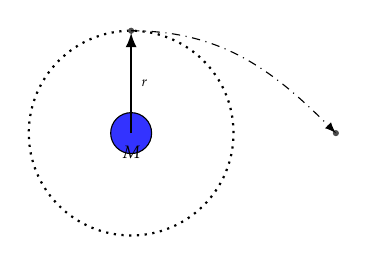
\begin{tikzpicture}[scale=1.3]
      \draw[fill=blue!80](0,0) circle(0.2) node[midway,below]{\tiny $M$};
      \draw[dotted,thick] (0,0) circle(1);
      \fill[black!70](0,1) circle(.03);
      \draw[->,thick](0,0)--(0,.98) node[midway,right]{\tiny $r$};
      \fill[black!70](2,0) circle(.03);
      \draw[->,dash dot](0,1) to[out=0,in=135](2,0);
    \end{tikzpicture}
    \hspace{.3in}
    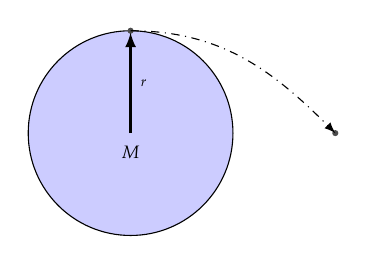
\begin{tikzpicture}[scale=1.3]
      \draw[fill=blue!20] (0,0) circle(1) node[midway,below]{\tiny $M$};
      \fill[black!70](0,1) circle(0.03);
      \draw[->,thick](0,0)--(0,.98) node[midway,right]{\tiny $r$};
      \fill[black!70](2,0) circle(0.03);
        \draw[->,dash dot](0,1) to[out=0,in=135](2,0);      
    \end{tikzpicture}
  \end{center}
  The difference is that the object in orbit (left) already has orbital speed
  $v_\text{orb}$, so escaping from that orbit requires only an additional
  speed of
  
  \eq{-.2in}{
    \Delta v=v_\text{esc}-v_\text{orbit}=(\sqrt{2}-1)v_\text{orbit}
  }
  \begin{itemize}
  \item What if $v_\text{orbit}<v<v_\text{esc}$?
  \item What if $v<v_\text{orbit}$?
  \end{itemize}
\end{frame}



\begin{frame}{Non-Circular Orbits}
  \centering
  \pic{.6}{newton-cannon-orbital-types-Seeds}
\end{frame}



\subsection{Orbital Energies}

\begin{frame}{Orbital Energies}
  We can obtain the \textbf{orbital kinetic energy} in a perfectly circular
  orbit by using the orbital speed in our expression of kinetic energy:

  \eq{-.2in}{
    K_\text{orb}=\frac12mv_\text{orb}^2=\frac12m
    \left(\sqrt{\frac{GM}{r}}\right)^2=\boxed{\frac{GMm}{2r}}
  }

  We already have an expression for gravitational potential energy:

  \eq{-.15in}{
    U_g=-\frac{GMm}{r}=-2K_\text{orb}
  }
\end{frame}



\begin{frame}{Orbital Energies}
  \vspace{-.1in}The \textbf{total orbital energy} is the sum of $K$ and $U_g$:

  \eq{-.15in}{
    E_T=K_{\text{orb}}+U_g=-\frac{GMm}{2r}=-K_{\text{orb}}
  }

  Note the relationship:

  \eq{-.2in}{
    K=-\frac12U_g=-E_T
  }

  You are unlikely to encounter this in an AP exam, but this relationship, when
  applied to \emph{electrostatic} force, was crucial in developing the first
  model for the hydrogen atom
\end{frame}



\begin{frame}{Binary System}
  \begin{columns}
    \column{.45\textwidth}
    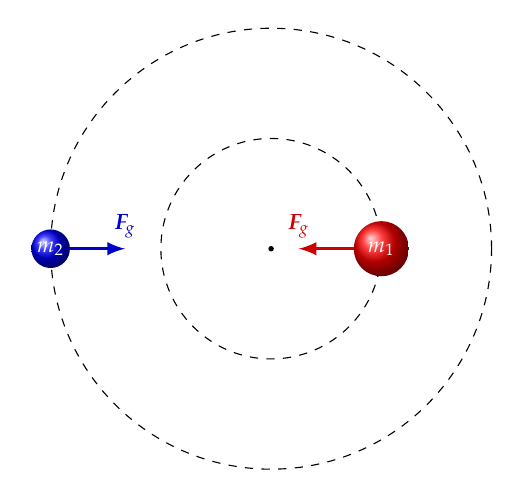
\begin{tikzpicture}[scale=.35]
      \fill(0,0) circle(.1);
      \draw[dashed](0,0) circle(4);
      \draw[dashed](0,0) circle(8);
      \tikzstyle{balloon1}=[ball color=red];
      \tikzstyle{balloon2}=[ball color=blue];
      \shade[balloon1] ( 4,0) circle(1)  node[white]{\footnotesize $m_1$};
      \shade[balloon2] (-8,0) circle(.7) node[white]{\footnotesize $m_2$};
      \draw[very thick,->,blue!80!black](-7.3,0)--(-5.3,0)
      node[above]{\footnotesize $\bm{F}_g$};
      \draw[very thick,->,red!80!black](3,0)--(1,0)
      node[above]{\footnotesize $\bm{F}_g$};
    \end{tikzpicture}

    \column{.55\textwidth}
    In a binary star system, two stars orbit around their center of mass. Both
    have the same period, and the gravitational force provides the centripetal
    force, but this time, the distance to the center of motion is empty space.
  \end{columns}
\end{frame}

\end{document}
